\chapter{Device maintenance}

\section{File system}

The \verb|show file systems| command (Figure \ref{ShowFileSystem}) lists all of the available file systems. This command provides useful information such as the amount of available and free memory, the type of file system, and its permissions. Permissions include read only (ro), write only (wo), and read and write (rw), shown in the Flags column of the command output.\\

\begin{figure}[hbtp]
\caption{The output of 'show filesystems' command}\label{ShowFileSystem}
\centering
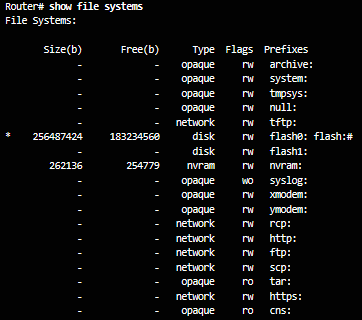
\includegraphics[scale=0.8]{pictures/ShowFileSystem.PNG}
\end{figure}

Notice that the flash file system also has an asterisk preceding it. This indicates that flash is the current default file system. The bootable IOS is located in flash; therefore, the pound symbol (\#) is appended to the flash listing.\\

The output of \verb|dir| command displays the contents of the current directory. Use \verb|dir <dir-name>| to view the content of the specified directory.\\

You can change the current directory using \verb|cd <dir>| command. The \verb|pwd| (present working directory) command shows you the name of the current directory. \\

In the \verb|flash| file system, the file with \verb|.bin| extension (usually the last listing) is the IOS file image that is running in RAM. 

\section{Back up and Restore}

\subsection{Using text file}

The steps to save a configuration using Tera Term follow:
\begin{enumerate}
\item On the File menu, click Log.
\item Choose the location to save the file. Tera Term begins capturing text.
\item After capture has been started, execute the \verb|show run| or \verb|show startup| command. Text displayed in the terminal window is directed to the chosen file.
\item When the capture is complete, select Close in the Tera Term: Log window.
\item View the file to verify that it was not corrupted.
\end{enumerate}

We can restore device configuration by copying the content of a text file to the terminal. Note that the text file requires editing to ensure that encrypted passwords are in plain text. Further, at the CLI, the device must be set at the global configuration mode to receive the commands from the text file being pasted into the terminal window.\\

When using Tera Term, follow these steps:
\begin{enumerate}
\item On the File menu, click Send file.
\item Locate the file to be copied into the device and click Open.
\item Tera Term pastes the file into the device.
\end{enumerate}

\subsection{Using TFTP}

You can use a service like Trivial File Transfer Protocol (TFTP) to remotely back up and restore files. Follow these steps to back up the running configuration to a TFTP server:

\begin{enumerate}
\item Enter the \verb|copy run tftp| command.
\item Enter the IP address of the host where the configuration file will be stored.
\item Enter the name to assign to the configuration file.
\item Press Enter to confirm each choice.
\end{enumerate}

\begin{verbatim}
R1# copy running-config tftp
Address or name of remote host []? 192.168.10.254
Destination filename [r1-confg]? R1-Jan-2016
Write file R1-Jan-2016 to 192.168.10.254? [confirm]
Writing R1-Jan-2016 !!!!!! [OK]
\end{verbatim}

Use these steps to restore the running configuration from a TFTP server:

\begin{enumerate}
\item Enter the copy tftp running-config command.
\item Enter the IP address of the TFTP server where the configuration file is stored.
\item Enter the name of the configuration file. For example, in the above example the file name was R1-Jan-2016.
\item Press Enter to confirm.
\end{enumerate}

\subsection{Using USB}

Images, configurations, and other files can be copied to or from the Cisco USB flash memory with the same reliability as storing and retrieving files using the Compact Flash card. In addition, modular integrated services routers can boot any Cisco IOS Software image saved on USB flash memory. 

\begin{verbatim}
R1# dir usbflash0:
Directory of usbflash0:/
1 -rw- 30125020 Dec 22 2032 05:31:32 +00:00 c3825-entservicesk9-mz.123-14.T
63158272 bytes total (33033216 bytes free)
\end{verbatim}

When backing up to a USB port, it is a good idea to issue the show file systems command to verify that the USB drive is there and confirm the name (Figure \ref{USB}). In this case, the USB has a name of \verb|usbflash0|

\begin{figure}[hbtp]
\caption{Verifying the USB drive is available}\label{USB}
\centering
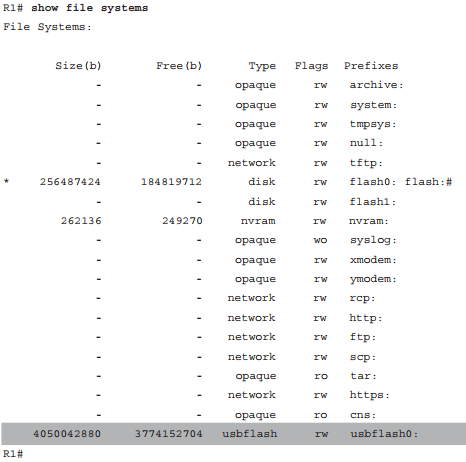
\includegraphics[scale=0.8]{pictures/USB.PNG}
\end{figure}

Use \verb|copy run usbflash0:/| command to copy the configuration file to the USB. To restore configuration from a USB, it is necessary to edit the file in USB with a text editor. Assuming the file name is \verb|R1-Config|, use the command \verb|copy usbflash0:/R1-Config run| to restore a running configuration.

\section{Password recovery}

Console access to the device using terminal emulator software on a PC is required for password recovery. With console access, a user can access the ROMMON mode by using a \emph{break sequence} during the bootup process or removing the external flash memory when the device is powered off.\\

Password recovery procedures on all devices follow the same principle:

\begin{enumerate}
\item Enter ROMMON mode

\item Change the configuration register to \verb|0x2142| (use \verb|confreg 0x2142| command) and reboot the device (use \verb|reset| command)

\begin{verbatim}
Readonly ROMMON initialized
monitor: command "boot" aborted due to user interrupt

rommon 1 > confreg 0x2142
rommon 2 > reset

System Bootstrap, Version 15.0(1r)M9, RELEASE SOFTWARE (fc1)
Technical Support: http://www.cisco.com/techsupport
Copyright (c) 2010 by cisco Systems, Inc.
<output omitted>
\end{verbatim}

\item After the device has finished rebooting, copy the startup configuration file to the running configuration file, use \verb|copy startup run| command. DO NOT enter \verb|copy run startup| because this command erases your original startup configuration.

\item Because you are in privileged EXEC mode, you can now configure all the necessary passwords.

\item After the new passwords are configured, change the configuration register back to \verb|0x2102| using the \verb|config-register 0x2102| global configuration mode command

\item Save the new configuration using \verb|copy run startup| command

\item Reload the device
\end{enumerate}

\textbf{ROMMON mode} enables an administrator to access flash memory, format the flash file system, reinstall the IOS, recover a lost password or change the configuration register. The configuration register instructs the router how to boot up. For example, when the configuration register is \verb|0x2142|, the device ignores the startup config file during startup. The default configuration register is \verb|0x2102|.

\section{IOS image}

\subsection{Naming convention}

Cisco Integrated Services Routers Generation Two (ISR G2) supports \emph{Services on Demand} through the use of software licensing. Each router is shipped with the same \emph{universal image}. The IOS features are enabled in the universal image via licensing keys.\\

There are two types of universal images supported in ISR G2:

\begin{itemize}
\item \textbf{With universalk9 in the name:} offer all Cisco IOS features

\item \textbf{With universalk9\_ npe in the name:} Not support strong cryptography such as payload cryptography.
\end{itemize}


The Cisco IOS image file has special naming convention. The \verb|show flash| command displays all files stored in flash memory including IOS image:

\begin{verbatim}
c1900-universalk9-mz.SPA.152-4.M3.bin
\end{verbatim}

\begin{table}[hbtp]
\centering\caption{Cisco IOS image naming convention}
\begin{tabular}{ll p{12cm} }
\toprule
\head{Part} & \head{Example} & \head{Explanation} \\
\midrule

Image name & \verb|c1900| & Identify the platform. In this example, the platform is Cisco 1900 router.\\

Image designation & \verb|universalk9| & The two designations for an ISR G2 are \verb|universalk9| and \verb|universalk9_npe|. \\

Status & \verb|mz| & Indicates where the image runs and if it is compressed. In this example, the image is running in RAM and is compressed.\\

Signature & \verb|SPA| & Digitally signed by Cisco\\

Version & \verb|152-4.M3| & Major release (15), minor release (2), maintenance release (4), maintenance rebuild number (3). The M indicates this is an extended maintenance release.\\

File extension & \verb|bin| & This extension indicates that this file is a binary executable file.\\

\bottomrule
\end{tabular}
\end{table}

The most common designation for memory location and compression format is \verb|mz|. The first letter indicates the location where the image is executed on the router. The locations can include: \verb|f| (flash), \verb|m| (RAM), \verb|r| (ROM), and \verb|l| (relocatable). The compression format can be either \verb|z| for zip or \verb|x| for mzip. 

\subsection{IOS image and TFTP server}

To create a backup of the Cisco IOS image to a TFTP server, perform the following three steps:

\begin{enumerate}
\item Ping TFTP server to test connectivity
\item Use \verb|show flash0:| command to determine the size of image file
\item Verify that TFTP server has sufficient disk space to accommodate the image file
\item Copy the image to TFTP server using \verb|copy flash0: tftp:|
\item Answer the prompted questions
\end{enumerate}

We can upgrade software in Cisco router by copying IOS image from TFTP server to the device:

\begin{enumerate}
\item Ping TFTP server to test connectivity
\item Use \verb|show flash0:| command to determine the size of image file
\item Verify that TFTP server has sufficient disk space to accommodate the image file
\item Copy the image to TFTP server using \verb|copy tftp: flash0:|
\item Answer the prompted questions
\end{enumerate}

\subsection{The boot system command}

To upgrade to the copied IOS image after that image is saved on the router's flash memory, configure the router to load the new image during bootup using the \verb|boot system| command

\begin{verbatim}
R1(config)# boot system flash0://c1900-universalk9-mz.SPA.152-4.M3.bin
\end{verbatim}

After the router has booted, to verify the new image has loaded, use the \verb|show version| command.\\

Several boot system commands can be entered in sequence to provide a fault-tolerant boot plan. If there are no boot system commands in the configuration, the router defaults to loading the first valid Cisco IOS image in flash memory and running it.

\section{Software licensing}

\subsection{Licensing key}

Recall that each device ships with the same universal image. Technology packages are enabled in the
universal image via Cisco IOS Software Activation licensing keys. \\

Each licensing key is unique to a particular device and is obtained from product ID, serial number of the router and a \emph{Product Activation Key (PAK)}. Cisco provides PAK at the time of purchase. \\

The IP Base is installed by default. Other technology Data, UC (Unified Communication), and SEC (Security) are enabled using licensing keys.\\

Use the \verb|show license feature| command to view the technology package licenses and feature licenses supported on the router.

\subsection{Licensing process}

A permanent license is a license that never expires. Evaluation license, known as a temporary license, allows customers to try a new software package. If customers want to permanently activate a software package or feature on the router, they must get a new software license.\\

There are three steps to permanently activate a new feature on the router:

\begin{enumerate}
\item Purchase the feature to install. Software Claim Certificates are used for licenses that require software activation. The claim certificate provides the PAK and Cisco EULA. PAK , an 11-digit alphanumeric key, serves as a receipt to obtain a license. A PAK
is not tied to a specific device until the license is created. 

\item Obtain license file using either CLM\footnote{Cisco License Manager, a free software application deploying Cisco licenses across networks} or Cisco License Registration Portal\footnote{web-based for getting and registering individual software licenses}. Then the license information is sent via email to install the license file. The license file is an XML  text file with a \textbf{.lic} extension.

\item Use \verb|license install <store-location>| to install license file

\begin{verbatim}
R1# license install flash0:seck9-C1900-SPE150_K9-FHH12250057.xml
\end{verbatim}

\item Reboot the router

\item Verify license using \verb|show license| and \verb|show version| command.
\end{enumerate}

Both of these processes require a PAK number and a unique device identifier (UDI). UID is the combination of Product ID (PID), Serial number (SN) and hardware version. The SN is an 11-digit number that uniquely identifies a device. The PID identifies the type of device. The UDI can be displayed using \verb|show license udi|.\\

\subsection{Activate an Evaluation license}

Evaluation licenses are replaced with RTU\footnote{Evaluation Right-to-Use licenses} after \textbf{60 days} (i.e. expired). These licenses are available on the honor system and require customer's acceptance of EULA. The \verb|license accept end user agreement| in global configuration mode is used to configure a one-time EULA acceptance for all IOS features. \\

Suppose you want to activate Data package on a Cisco 1900 router, the following command should be executed:

\begin{verbatim}
R1(config)# license boot module c1900 technology-package datak9
\end{verbatim}

Technology package names are \verb|ipbasek9|, \verb|securityk9|, \verb|datak9|, and \verb|uck9|.\\

Remember that the device has to reboot to activate new software package.

\subsection{Back up the license}

To copy all licenses in a device and store them in flash memory with the file name \verb|all_licenses.lic|, execute the following command:

\begin{verbatim}
R1# license save flash0:all_licenses.lic
\end{verbatim}

\subsection{Uninstall a permanent license}

Perform the following steps to completely uninstall an active permanent license:

\begin{enumerate}
\item Disable technology package, then reboot

\begin{verbatim}
R1(config)# license boot module c1900 technology-package seck9 disable
R1(config)# exit
R1# reload
\end{verbatim}

\item Clear technology package license

\begin{verbatim}
R1# license clear seck9
\end{verbatim}

\item Remove the \verb|license boot module| command in step 1, and then reload.

\begin{verbatim}
R1(config)# no license boot module c1900 technology-package seck9 disable
R1(config)# exit
R1# reload
\end{verbatim}
\end{enumerate}